\documentclass[letterpaper,10pt]{article}

\usepackage{titling}
\usepackage{listings}
\usepackage{url}
\usepackage{setspace}
\usepackage{subfig}
\usepackage{sectsty}
\usepackage{pdfpages}
\usepackage{colortbl}
\usepackage{multirow}
\usepackage{multicol}
\usepackage{relsize}
\usepackage{amsmath}
\usepackage{wasysym}
\usepackage{fancyvrb}
\usepackage{amssymb}
\usepackage{ifsym}
\usepackage{amsmath,amssymb,amsthm,graphicx,xspace}
\usepackage[titlenotnumbered,noend,noline]{algorithm2e}
\usepackage[compact]{titlesec}
\usepackage{XCharter}
\usepackage[T1]{fontenc}
\usepackage{tikz}
\usetikzlibrary{arrows,automata,shapes,trees,matrix,chains,scopes,positioning,calc}
\tikzstyle{block} = [rectangle, draw, fill=blue!20, 
    text width=2.5em, text centered, rounded corners, minimum height=2em]
\tikzstyle{bw} = [rectangle, draw, fill=blue!20, 
    text width=4em, text centered, rounded corners, minimum height=2em]

\definecolor{namerow}{cmyk}{.40,.40,.40,.40}
\definecolor{namecol}{cmyk}{.40,.40,.40,.40}

\let\LaTeXtitle\title
\renewcommand{\title}[1]{\LaTeXtitle{\textsf{#1}}}


\newcommand{\handout}[5]{
  \noindent
  \begin{center}
  \framebox{
    \vbox{
      \hbox to 5.78in { {\bf ECE356: Database Systems } \hfill #2 }
      \vspace{4mm}
      \hbox to 5.78in { {\Large \hfill #4  \hfill} }
      \vspace{2mm}
      \hbox to 5.78in { {\em #3 \hfill} }
    }
  }
  \end{center}
  \vspace*{4mm}
}

\newcommand{\lecture}[3]{\handout{#1}{#2}{#3}{Lecture #1}}
\newcommand{\tuple}[1]{\ensuremath{\left\langle #1 \right\rangle}\xspace}

\addtolength{\oddsidemargin}{-1.000in}
\addtolength{\evensidemargin}{-0.500in}
\addtolength{\textwidth}{2.0in}
\addtolength{\topmargin}{-1.000in}
\addtolength{\textheight}{1.75in}
\addtolength{\parskip}{\baselineskip}
\setlength{\parindent}{0in}
\renewcommand{\baselinestretch}{1.5}
\newcommand{\term}{Winter 2018}

\singlespace


\begin{document}

\lecture{ 35 --- Recovery: Repair, Probability} {\term}{Jeff Zarnett}

\section*{Probabilistically Answering Queries}


Residues and repairs are not the only way to return consistent answers. When there are several options, as in Table~\ref{inconsistent1}, we can examine these options and make a determination of which is more likely. We form candidates - pretenders to the throne of the correct database -  by breaking up the possibilities for repair into all of their possible variants; in each candidate database, one tuple from each cluster is selected. We see that in the example of Table~\ref{inconsistent1}, both candidate databases will receive a probability of being the ``correct" database.

\begin{table}[h]\begin{center}
        \begin{tabular}{r | c  c} 
					salaries & employee\_name & salary \\ \hline
	           		 & J. Page  & 50 000 \\ 
	         		 & J. Page  & 80 000 \\ 
					 & V. Smith & 35 000 \\ 
					 & M. Stowe & 75 000 \\ 
        \end{tabular}
        \caption[Inconsistent Salaries Table]{Inconsistent Salaries Table~\cite{CQ}\label{inconsistent1}}
\end{center}\end{table}

\paragraph{Finding Consistent Answers}
Andritsos, Fuxman, and Miller in \cite{CA} take the approach of examining various probabilities of each tuple in a cluster being the correct answer. In the simplest solution, the database will just answer queries and attach the probability of the answer's correctness as another attribute of the tuple. Referring back to the salary example, below in Table~\ref{inconsistent2} is Table~\ref{inconsistent1} modified with the respective probabilities of each item:


\begin{table}[h]\begin{center}
        \begin{tabular}{r | c  c  c} 
					salaries & employee\_name & salary & probability\\ \hline
	           		 & J. Page  & 50 000 & 0.1 \\ 
	         		 & J. Page  & 80 000 & 0.9 \\ 
					 & V. Smith & 35 000 & 0.4 \\ 
					 & M. Stowe & 75 000 & 1 \\ 
        \end{tabular}
        \caption[Inconsistent Salaries Table with Probabilities]{Inconsistent Salaries Table with Probabilities \cite{CQ} \cite{CA}\label{inconsistent2}}
\end{center}\end{table}

If the query being asked were all the names of all employees making more than \$70~000, a probabilistic assessment would be performed to decide what certainty we could indicate the answers with. In the trivial case, M. Stowe's salary is certainly greater than \$70~000, since its probability is 1 (completely certain). Uncertainty enters the picture when examining the J. Page tuples. We note probability of his salary being \$80~000 is 0.9, so we include him in the return set and indicate the attached probability. If the query were names of employees making more than \$45~000, then we would return J. Page with probability 1, since the sum of the probabilities of the tuples wherein his salary exceeds \$45~000 is 1. 

Andritsos, Fuxman, and Miller simply modify the requested queries to include the probability attributes. If the original query was:\\
\texttt{SELECT s.employee\_name FROM salaries s WHERE s.salary > 70~000}\\
then the only changes are the addition of\texttt{SUM(s.probability)} and \texttt{GROUP BY s.employee\_name}, so that the rebuilt query reads:\\
\texttt{SELECT s.employee\_name, SUM(s.probability) FROM salaries s WHERE s.salary $>$ 70~000 \\ GROUP BY s.employee\_name}\\

In a more complex query, we simply multiply the probabilities. Consider the following query \cite{CA}: \\
\texttt{SELECT o.id, c.id FROM order o, customer c  WHERE o.cIdFk = c.id AND c.balance > 10000 } \\
This query is modified in the same way as that of the preceding paragraph, except the sum statement reads \texttt{SUM(o.probability * c.probability)} and the group statement is \texttt{GROUP BY o.id, c.id}.

\paragraph{Determining Probabilities}
The most pressing question is how we determine the probabilities. We note there are definite conditions attached to being able to determine these. See Figure \ref{formula} for the detailed breakdown of the procedure to map the tuples' probability to the interval [0, 1].

\begin{figure}[!h]
  \centering 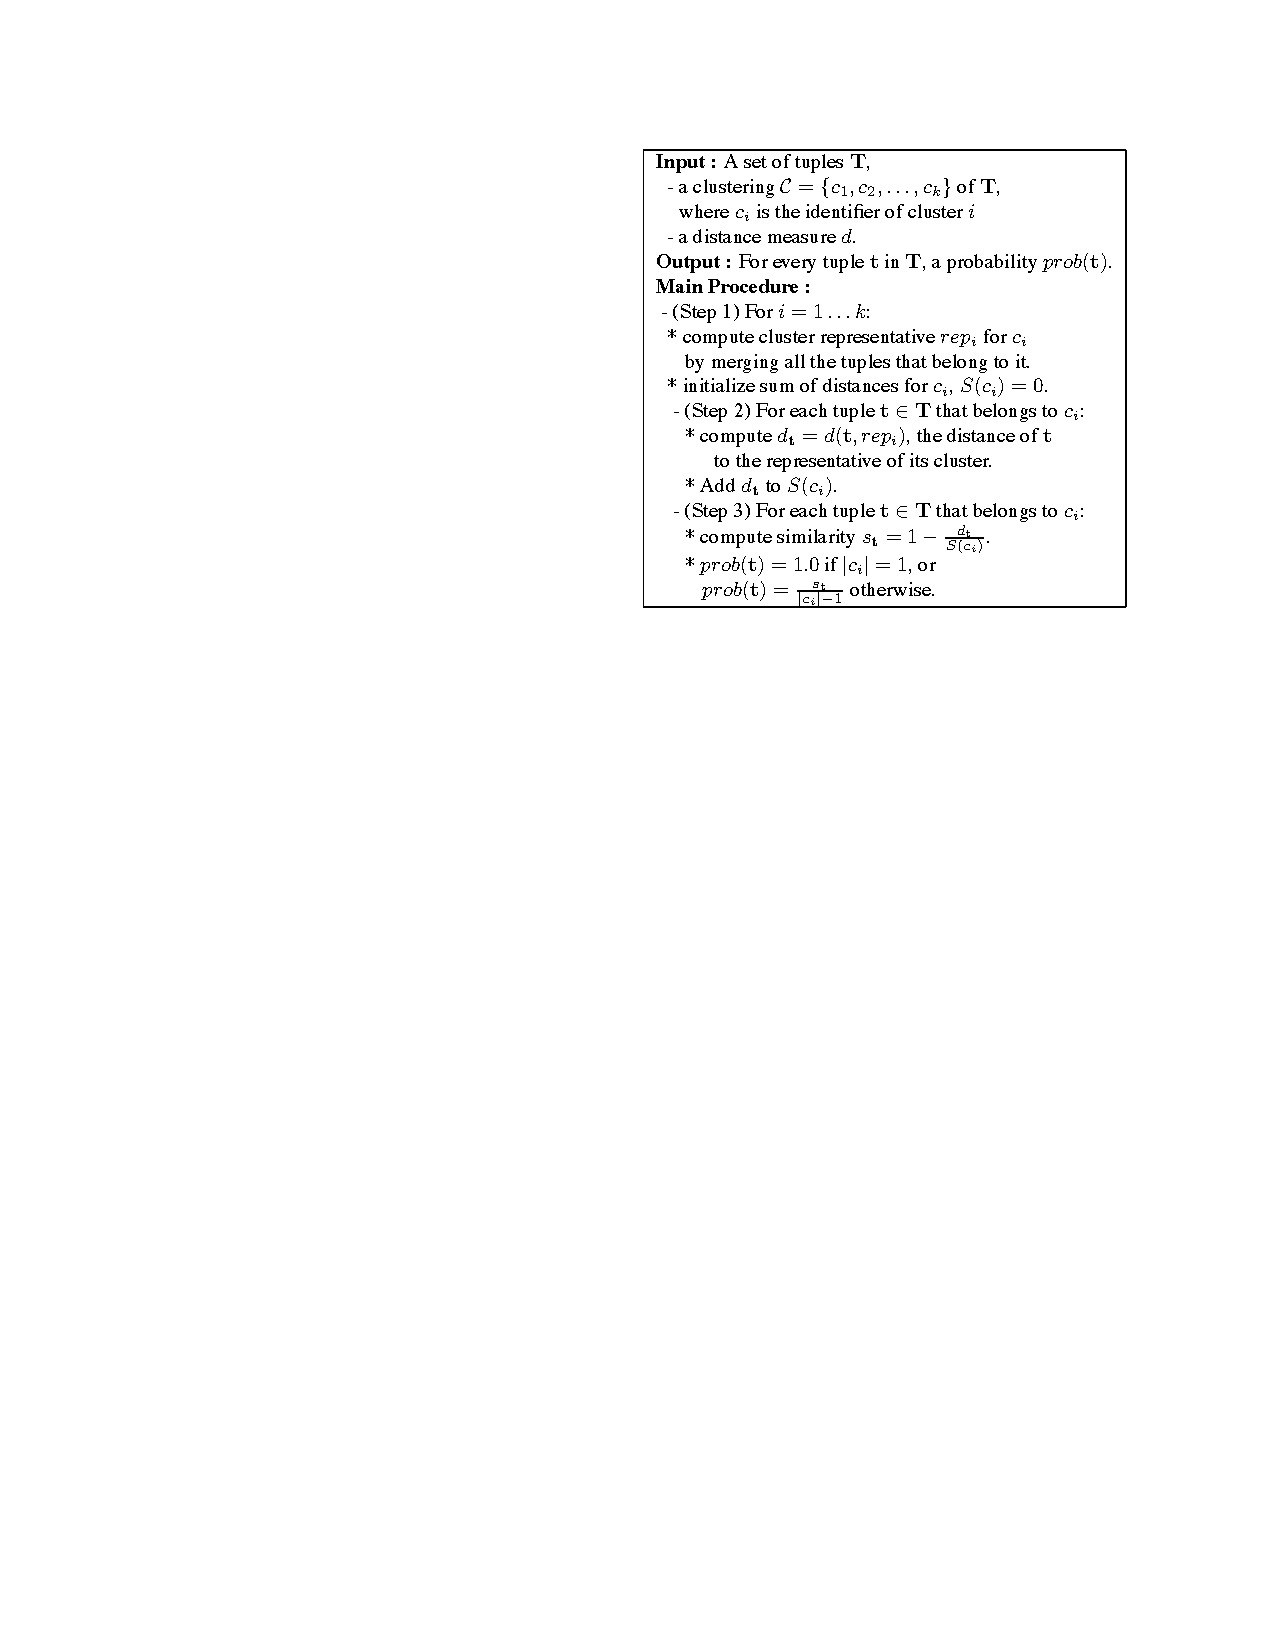
\includegraphics{images/formula.pdf}
  \caption[Tuple Probability Assignment Formula]{Tuple Probability Assignment Formula \cite{CA}}
  \label{formula}
\end{figure}

Though most of the algorithm is self-explanatory, some components merit clarification, also provided in \cite{CA}. Tuples within a cluster must be exclusive events, or the algorithm will fail. Representatives are determined by commonality. Representatives contain the most common features in the cluster, so the similarity between the tuples will give an indication of which tuple is most likely to be representative. To clarify, a short example, Table~\ref{rep}:

\begin{table}[h]\begin{center}
        \begin{tabular}{r | c  c  c  c } 
					customers & name & market\_segment & country & address\\ \hline
	           		 & Mary   & building & USA    & 123 Jones Ave. \\ 
	         		 & Mary   & banking  & Canada & 123 Jones Ave. \\ 
					 & Marion & banking  & USA    & 123 Jones Ave. \\ 
        \end{tabular}
        \caption[Inconsistent Customers Table]{Inconsistent Customers Table \cite{CA}\label{rep}}
\end{center}\end{table}

When examining this with a human's eyes, we might conclude that the most common values in the database are probably the correct ones, so the resultant representative tuple would show the customer Mary as part of banking in the USA with an address of 123 Jones Ave. The algorithm shown in Figure \ref{formula} follows this same intuition. The tuple we will consider correct is the one closest to the representative. For numerical data, similarity between two figures can be computed, and a pair can be more or less similar than another pair of figures (456 and 385 are more similar than 750 and 385). For data for which there is no obvious distance measure, we term them \textit{categorical data}, and we proceed using information loss as the distance metric \cite{CA}. Information loss is simply a measure of the difference between  the tuple in question and the representative. 

\paragraph{Analytical Shortcomings}

The strategy presented is imperfect, however, since we might fail to produce clean answers for some classes of query. Andritsos, Fuxman, and Miller present in \cite{CA} the following case as unable to succeed: \texttt{select c.id from order o, customer c  where o.quantity < 5 and o.cIdFk = c.id and c.balance > 25~000}. This fails because the join between \texttt{c} and \texttt{o} incorrectly double-counts some probabilities. Obviously, query rewriting cannot succeed for all cases, so the algorithm is limited to only those which we can reliably rewrite. Andritsos, Fuxman, and Miller argue -- without proof -- that  such un-rewritable queries occur only infrequently, and that the algorithm is still valid most of the time.

Overlooked in this analysis is determining how we might find a representative sample when it is not obviously in a majority-rules scenario. Given two prima facie equally plausible tuples, how do we decide which is the better choice to consider the representative? Whichever is picked to be the representative will not differ from the representative (by definition), so it will receive a probability of 1. Thus, whatever we (perhaps randomly) choose to be our representative is the eventual winner and will be considered correct. It is clear that we need to come to some decision, but reporting 100\% certainty about data which is, at best, 50\% certain is misleading. 

This analysis also equates popular with correct. If an incorrect answer appears in the database twice and a correct answer once, then the incorrect answer will be chosen and deemed correct, since it is more popular. That aside, there is not much that can be done about this problem; even a human observing the database might be more likely to conclude that the popular answer is the correct one, in the absence of additional, external knowledge.

\section*{Computational Complexity of Repair \& Probability}
Computational complexity is broken down into a short analysis on each of the methods detailed above. Each approach has its own properties. Computational complexity may disqualify a method from being practically useful, should it take too much time to reach a reasonable answer.

\paragraph{Repairing Databases}
Assuming that we are looking at repairs that are subsets of the original database, then repair checking is in polynomial time, for arbitrary constraints combined with acyclic dependencies \cite{CQ}. Should any of these constraints not hold, the problem is pushed into the realm of co-NP-complete problems, although additional orthogonal restrictions might lead to more polynomial time cases \cite{CQ}.

Having considered the spectre of computationally infeasible or impossible situations, Bertossi and Chomicki \cite{CQ} develop various methods of finding consistent answers without explicitly computing every possible repair to the database. One of the ways that they suggest is compact repair representation - use information present to construct an efficient representation of all the possible repairs, and use this representation to answer all queries. However, this is not explored in the paper.

\paragraph{Query Transformation} 
The process of query transformation in \cite{CQ} is shown to have a polynomial time computability of result tuples, as the transformed query will be first order as long as the original query is as well. In fact, because the query transformation does not require examining all the possible repairs, so we can evaluate a query with an exponential number of possible repairs in polynomial time.

\paragraph{Aggregate Query Transformation}
The approach presented in \cite{CQ} is to aggregate queries is to build a conflict graph; a standard graph with nodes and edges. In the graph, maximal independent sets - that is, sets that are the farthest apart in terms of data equality - represent possible repairs of the database. As long as there is at most one nontrivial constraint, all operators except \texttt{COUNT} are polynomial time. If there are many nontrivial constraints, then the problem of finding lower and upper bounds becomes NP-complete. The \texttt{COUNT} operation is always NP-complete, even in the case of a single nontrivial constraint. Finally, it is noted that the \texttt{AVG} function's polynomial time algorithm is iterative, and cannot be formulated using SQL. 

Under special circumstances, Bertossi and Chomicki found some better behaviour for the \texttt{COUNT} function, but even approximating is difficult; the concept of a maximal independent set reportedly has bad approximation properties.

\paragraph{Probabilistic Complexity}
Andritsos, Fuxman, and Miller include in \cite{CA} a note on the computational complexity of their work.  specifically a graph showing the performance as the size of the database grows, reproduced here as Figure \ref{CAPerformance}:

\begin{figure}[!h]
  \centering 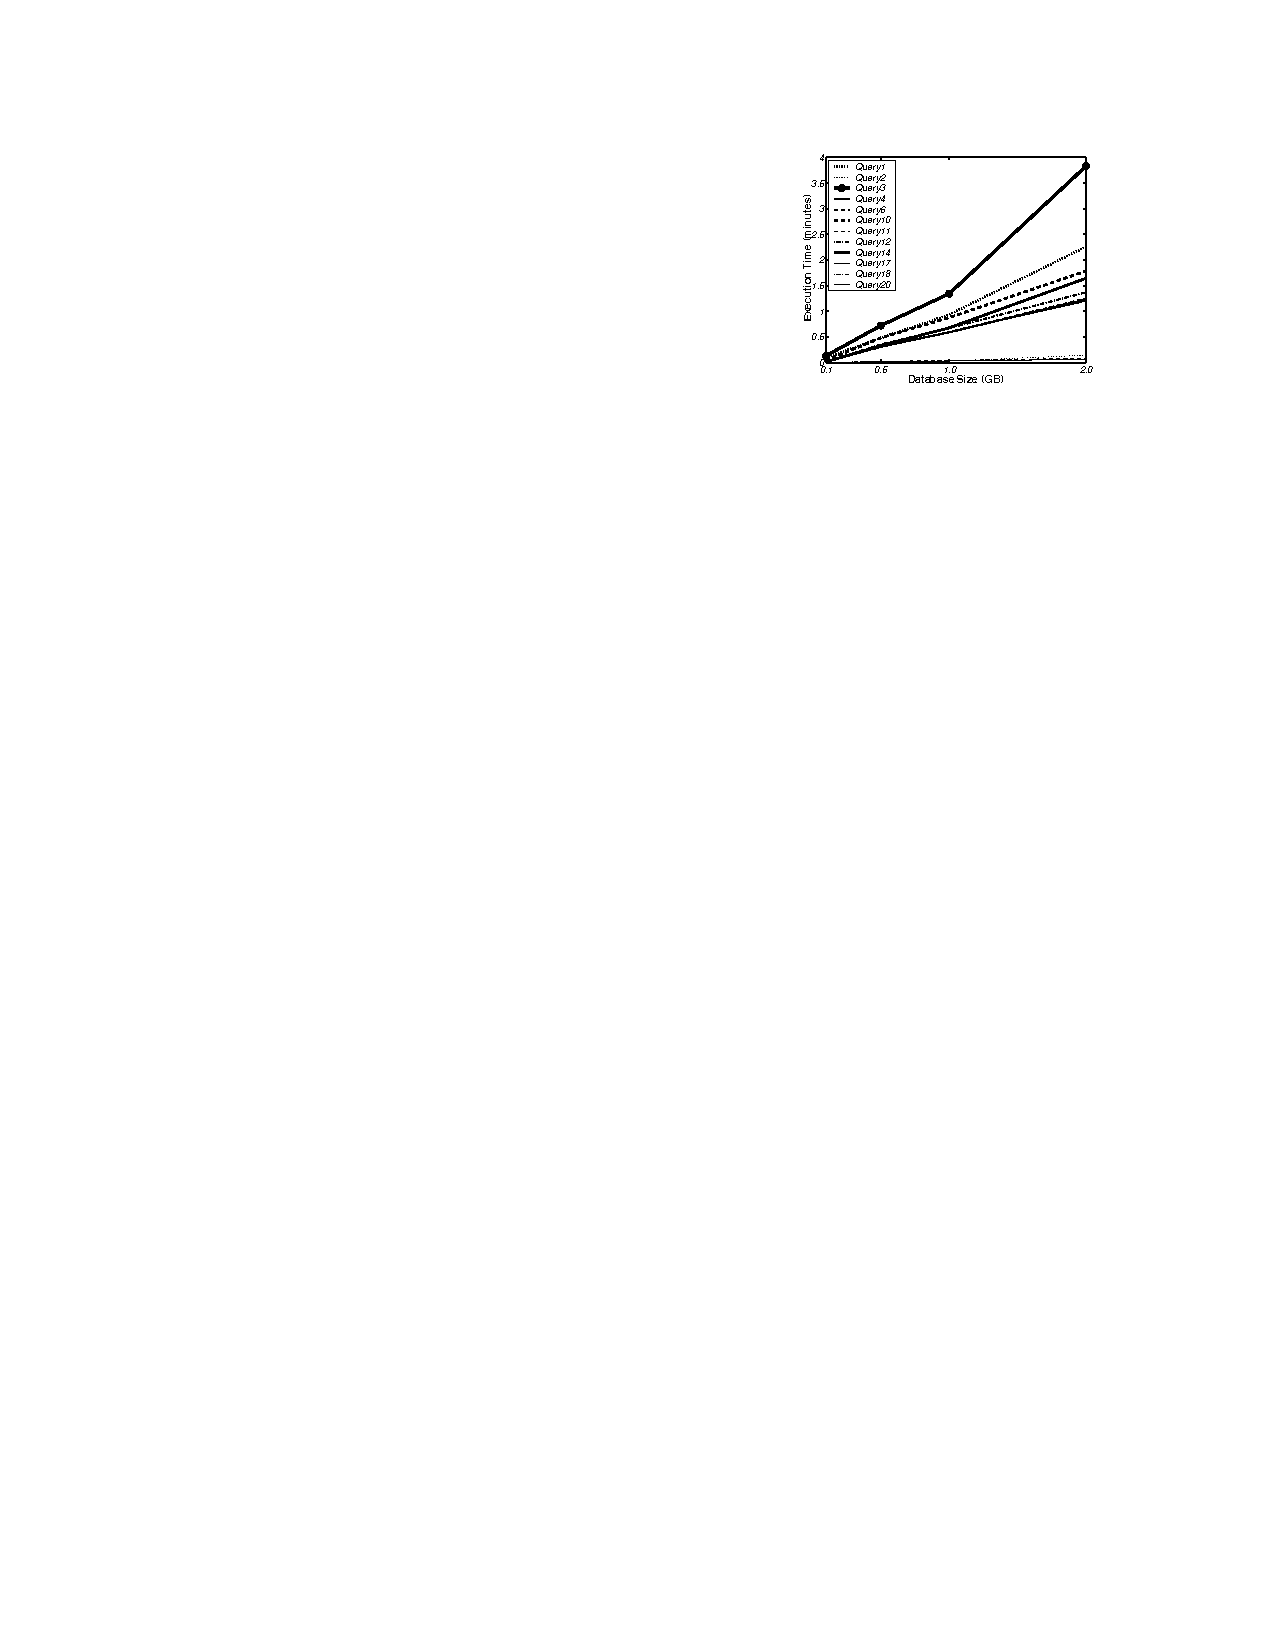
\includegraphics[width=4in]{images/CAPerformance.pdf}
  \caption[The Effect of Database Size on Probabilistic Evaluation]{The Effect of Database Size on Probabilistic Evaluation \cite{CA}}
  \label{CAPerformance}
\end{figure}

It is clear from a cursory examination that the behaviour of the queries is linear, with the exception of some corner cases (like Query 3). However, they sidestep the issue that the number of candidate databases is possibly exponential - if there are \textit{n} inconsistencies each with clusters of size \textit{m}, the total possibilities might be as large as $n^{m}$. Computing probabilities for such a set might be exceedingly difficult, but the whole issue is glossed over with a single comment.

\subsection*{Future Work \& Suggestions}

In \cite{CQI}, Arenas, Bertossi, and Chomicki warn that their proofs of termination and completeness properties of the query transformation are only preliminary and partial. Surely this will be addressed in the future. They also find that completeness for disjunctive and and existential queries, they will need to move beyond simple query transformations. In addition, they do not yet have upper bounds on the size of the transformed query, and they lack some complexity information on different classes of query. This particular paper (\cite{CQI}) is a more detailed examination of some sections of \cite{CQ}), with two authors in common, so suggestions for improving it are combined with that of its successor.

Database repairs examined in the \cite{CQ} fashion are based on differences against the whole tuple and does not permit modifying attributes of tuples. Bertossi and Chomicki suggest that a \textit{flexible} (attribute-level) repairs. They further identify majority-based approaches to consistency, which is very similar to how the probabilistic approach decides what to do.

Further in that paper, the section on logic programs to compute database repairs is rather light on details and seems mostly an aggregation of examples. We suggest that the paper might be improved by including more detail on the subject, since a lot has been left out, or reducing the amount of space dedicated to what is clearly a side point implementation detail. 

In this same vein, there is a note about computationally constructing compact repair representations, yet there is not much talk about how we might do this, aside from a side note about placing \texttt{null} into a field when there are infeasibly many repairs. We suggest expanding compact repair representations, or clarifying the note about them (which implies that there is a wealth of information on the topic coming).

The probabilistic paper presents no future extensions or future directions to its work. As suggestions for them, they could certainly investigate the computational complexity further. Specifically, why some cases are more difficult than others to handle (see query 3 in Figure \ref{CAPerformance}). They also appear to lack a strategy for dealing with a large set of inconsistencies. 

Noting the scenario in which 50\% certain data may be reported 100\% certain, my suggestion for such forced-guess scenarios is to report the uncertainty associated with this answer and confess that we cannot find any better solution without additional input.

Finally, the set of queries that they cannot rewrite is claimed to be small, but no proof or evidence is offered to convince the reader that this is really the case. Surely a subsection or followup would be rather more persuasive than simply taking it on faith.

\subsection*{Conclusion}

There appears to be no single right answer when dealing with an inconsistent database. However inconsistent it may be, it is unlikely that we will be able to unequivocally say what is correct and what is not. All of the examined options present viable alternatives to solving the problem, but they can easily slip into computational infeasibility in the event of complex constraints or a great number of inconsistencies. With these techniques, we can certainly get back consistent answers to our queries. The success of aggregate queries is less certain, but the chances are still reasonable.

Some techniques report uncertainties, and others ignore anything about which we are uncertain. Ultimately, how to handle the situations comes down to the decision of the database administrator or designer. He or she will need to choose the solution he or she feels appropriate to the situation. 



\bibliographystyle{alphaurl}
\bibliography{356}


\end{document}
